\documentclass{bioinfo}

%\usepackage[sort,numbers]{natbib}

\usepackage{booktabs}
\usepackage{color}
\usepackage[dvipsnames]{xcolor}

\usepackage[capitalise]{cleveref}
%\usepackage[noend]{algorithm2e}
\usepackage[ruled,noend]{algorithm2e}
\newcommand\mycommfont[1]{\scriptsize\rmfamily%\textcolor{blue}
	{#1}}
\SetCommentSty{mycommfont}
\SetEndCharOfAlgoLine{.}
%\crefname{algocf}{alg.}{algs.}
\crefname{algocf}{Algorithm}{Algorithms}
\Crefname{algocf}{ALG}{ALG}

\usepackage{graphicx}
\usepackage{tikz}
\usepackage{pgfplots}
\usepackage{pgfplotstable}

\usepgfplotslibrary{groupplots}
\pgfplotsset{compat=newest}
\pgfplotsset{
	log x ticks with fixed point/.style={
		xticklabel={
			\pgfkeys{/pgf/fpu=true}
			\pgfmathparse{exp(\tick)}%
			\pgfmathprintnumber[fixed relative, precision=3]{\pgfmathresult}
			\pgfkeys{/pgf/fpu=false}
		}
	},
	log y ticks with fixed point/.style={
		yticklabel={
			\pgfkeys{/pgf/fpu=true}
			\pgfmathparse{exp(\tick)}%
			\pgfmathprintnumber[fixed relative, precision=3]{\pgfmathresult}
			\pgfkeys{/pgf/fpu=false}
		}
	}
}

\usepackage[group-separator={\,}]
{siunitx}
\pgfkeys{/pgf/number format/.cd,1000 sep={\,}}
%\DontPrintSemicolon
%\usepackage{hyperref}

\copyrightyear{2018} \pubyear{2018}

\access{Advance Access Publication Date: 01 January 2018}
\appnotes{Manuscript Category: article}

\begin{document}
\firstpage{1}

\subtitle{Sequence clustering}

\title[FgClust]{FgClust, a fast and scalable algorithm for generating high-quality clusters of biological sequences}
\author[XiaoFei Zhao \textit{et~al}.]{
	XiaoFei Zhao\,$^{\text{\sfb 1,}*}$
	%, Co-Author\,$^{\text{\sfb 2}}$ 
	and Shing Hei Zhan\,$^{\text{\sfb 1,}}$}
\address{$^{\text{\sf 1}}$Bioinformatics Department, Fusion Genomics Corporation, Burnaby, V5A 4W9, Canada 
%	and \\
%$^{\text{\sf 2}}$Department, Institution, City, Post Code,
%Country.
}

\corresp{$^\ast$To whom correspondence should be addressed.}

\history{Received on XXXXX; revised on XXXXX; accepted on XXXXX}

\editor{Associate Editor: XXXXXXX}

\abstract{\textbf{Motivation:}
Many sequence clustering algorithms have been designed for sequence databases that grow exponentially fast.
However, no clustering algorithm is sensitive, specific, fast, and scalable, all at the same time.
A more sensitive (specific) clustering algorithm is more likely to partition sequences with the same (different) biogical propertie(s) into the same (different) cluster(s), respectively.
Important biogical properties include three-dimensional structures (i.e., protein structures in Protein Data Bank (PDB)), and biologial functions (i.e., Pfam and Rfam families).
\\
\textbf{Results:}
We developed FgClust, a novel multi-threaded algorithm for clustering biological sequences.
FgClust uses clique-aware all-versus-all search instead of greedy incremental update, a reasonable number of centroid-sequence candidates per indexed k-mer group instead of either an unlimited number of or only one such candidate, and the length of non-centroid sequence minus infix Levenshtein distance instead of sequence identity.
We evaluated FgClust, Linclust, MMSeqs2, CD-HIT, and kClust by using
five versions of UniRef100 released between July 2004 and January 2017, 
the protein structures deposited into PDB exclusively before January 2\textsuperscript{nd} 2017, and Pfam-A-seed 31.0.
We evaluated FgClust, VSEARCH, and CD-HIT-EST by using Rfam 12.3.
Our evaluations show that FgClust always achieves the fastest runtime except Linclust and the best sensitivity-specificity trade-off without any exception.
Linclust is approximately three times faster but generates up to more than 150\% more clusters than FgClust.
The observed runtime of FgClust increases linearly with input size.
In one day, FgClust can cluster hundreds of millions of proteins, such as the ones in each expected release of UniProt in the next few years, into tens of millions of high-quality clusters.
\\
\textbf{Availability:} FgClust is available under the MIT license at \href{https://github.com/zhaoxiaofei/fgclust}{https://github.com/zhaoxiaofei/fgclust}\\
\textbf{Contact:} %\href{xzhao@fusiongenomics.com}{xzhao@fusiongenomics.com} or
\href{cndfeifei@hotmail.com}{cndfeifei@hotmail.com}
\\
\textbf{Supplementary information:} Supplementary data are available at \textit{Bioinformatics}
online.}

\maketitle

\section{Introduction}

Sequence clustering is a common step in bioinformatics pipelines to reduce sequence redundancy (e.g., construction of the non-redundant protein sequence database UniProt Reference Clusters (UniRef) at 50\% and 90\% sequence-identity cutoffs \citep{suzek2007uniref}), to predict biological function (e.g., sequence assignment to known protein families \citep{finn2016pfam}), and to identify novel and/or unique sequences (e.g., detection of orphan genes \citep{prabh2016orphan}). As molecular sequence data accumulate at an accelerating pace from numerous genome and metagenome sequencing efforts, the availability of scalable and reliable sequence clustering algorithms has become increasingly critical.

The reliability of a clustering algorithm is measured by its sensitivity and specificity.
A more sensitive clustering algorithm generates fewer clusters of higher average cluster size.
A more specific clustering algorithm generates clusters such that sequences in the same cluster typically share more biological properties.
A clustering algorithm achieves better sensitivity-specificity trade-off if it exhibits either better sensitivity at a given specificity or better specificity at a given sensitivity.
An improved sensitivity-specificity trade-off yields higher-quality clusters, and vice versa.
Higher-quality clusters reduce manual-curation efforts as well as errors in the downstream analysis of the clusters.


Cluster quality depends on specificity that needs to be evaluated with respect to some biological properties.
Two % of 
important biological properties are three-dimensional structure and biological function.
Example applications of the study of three-dimensional structure include
discovery and design of new drugs  \citep{kryger1999structure}, 
diagnosis of disease \citep{gniadecka2004melanoma}, and
prediction of biological function \citep{berg2002protein}.
Example applications of the study of biological function include
increase in crop yield \citep{xu2011functions},
therapy for disease \citep{cowen2009harnessing,egen2002ctla}, and
prevention of disease \citep{kris2004bioactive}.

The Protein Data Bank (PDB) database contains experimentally determined three-dimensional protein structures \citep{berman2006protein}.
The Pfam-A-seed and Rfam-seed datasets are manually checked protein and RNA families, respectively, such that sequences in the same family perform the same biological function \citep{finn2016pfam,nawrocki2014rfam}.
Thus, we used PDB protein structures, Pfam-A-seed families,  Rfam-seed families for evaluating specificity and thereby cluster quality.

Numerous computational techniques have been explored to improve runtime and/or cluster quality.
If two sequences do not share a certain percentage of short words (i.e., k-mers), then the sequence identity between these two sequences is likely to fall below a certain specified threshold.
The popular program CD-HIT assumes that these two sequences are in different clusters and skips computing the alignment between these two sequences \citep{li2002tolerating}.
This skipping significantly improves runtime without significantly sacrificing sensitivity.
Given multiple targets ordered by decreasing percentage of short words shared with a query, if the sequence identity between the query and each of the first few targets is less than a threshold, then the sequence identity between the query and each of the remaining targets is also likely to be less than a threshold.
Another popular program, UCLUST, assumes that the remaining targets cannot be clustered with the query and therefore skips them altogether \citep{edgar2010search}.
This skipping also significantly improves runtime without significantly sacrificing sensitivity.
Two different short words having a high alignment score can still be considered as matching to each other.
The sequence profile of a cluster is more sensitive than the centroid of the cluster for integrating sequences into the cluster.
kClust uses similarity-based short-word match and sequence profile to improve sensitivity without significant sacrificing specificity and runtime \citep{hauser2013kclust}.
kClust, MMSeqs, and MMSeqs2 all use similar ideas \citep{hauser2013kclust,hauser2016mmseqs,steinegger2017mmseqs2}.

Functionally important sequences (or substrings thereof) tend to be evolutionarily conserved.
Consequently, the same conserved k-mers are usually shared by sequences in the same family.
Linclust attempts to find sequence family from such conserved k-mers \citep{steinegger2017linclust}.
More specifically, 
Linclust indexes k-mers in input sequences, 
selects only one centre sequence per k-mer,
and then aligns each input sequence to only a constant number of centre sequences that share at least one k-mer with the input sequence \citep{steinegger2017linclust}.
In this way, the worst-case runtime of Linclust scales linearly with the number of input sequences.
However, k-mer match does not always imply biological similarity.
In fact, a k-mer match may occur by chance.
Therefore,
even if the centre sequence of a k-mer is not biological similar to the non-centre sequences of the k-mer, 
some of the non-centre sequences can still be biologically similar to each other.
Suppose that k-mer length is fixed and that the number of input sequences increases linearly.
Then, for each input sequence,
the number of k-mer matches to other input sequences by chance increases linearly.
However,
the average cluster size increases sub-linearly \citep[Fig. 3]{suzek2014uniref},
and only sequences in the same cluster are supposed to be biologically similar to each other.
Therefore,
for each input sequence,
the number of k-mer matches to other input sequences by biological similarity increases sub-linearly.
Therefore, the number of k-mer matches by chance asymptotically outgrows the number of k-mer matches by biological similarity.
As a result, as the number of input sequences increases, 
the sensitivity of Linclust decreases (\cref{fig:uniref}) so that the quality of the clusters generated by Linclust decreases.

So far, no algorithm can generate high-quality clusters in linear time at a reasonable speed in practice.
To address some of the deficiencies,  we developed a novel sequence-clustering algorithm named FgClust.
FgClust is enhanced by novel heuristics and algorithmic techniques that result in linear runtime with improved cluster quality.
%without sacrificing sensitivity, specificity, or cluster quality. 
Our main algorithmic novelties are the use of (1) clique-aware all-versus-all search instead of greedy incremental update, 
%(2) min-hash values instead of short words, and 
(2) a limited number of centroid-sequence candidates per indexed k-mer instead of either an unlimited number of or only one centroid-sequence candidates per indexed k-mer, and
(3) Levenshtein distance instead of a sequence alignment score (e.g., from a pairwise Smith-Waterman alignment). Moreover, we improved existing techniques, such as greedy set cover \citep{steinegger2017mmseqs2} and pruning of sorted hit candidates \citep{edgar2010search}, and combined these improved techniques with our algorithmic novelties.

Here, we demonstrated that FgClust can cluster hundreds of millions of sequences in one day on a typical server and produce biologically faithful sequence clusters. In benchmark experiments, we found that FgClust outperforms almost all published methods (Linclust, MMSeqs2, CD-HIT, kClust, and VSEARCH). FgClust always achieves better sensitivity without compromising specificity and better specificity without compromising sensitivity. In terms of runtime, FgClust exceeds all the other methods except Linclust, which finishes approximately three times as fast as FgClust in the benchmark data sets. Importantly, however, FgClust generates fewer sequence clusters of higher quality than Linclust and the other methods. Overall, FgClust is a novel sequence clustering method that offers outstanding scalability while putting emphasis on sequence cluster quality. FgClust is publicly available at \href{https://github.com/zhaoxiaofei/fgclust}{https://github.com/zhaoxiaofei/fgclust}.

%\enlargethispage{12pt}

\begin{methods}
	
\section{Methods}

\SetKwInOut{Parameter}{Parameter}

\subsection{Clique-aware all-versus-all search}
\label{subsec:clique-aware}
\Citet{li2001clustering} introduced the notion of greedy incremental update.
Greedy incremental update involves visiting each sequence (typically in order of decreasing sequence length) and then either forming a new cluster with each visited sequence or assigning it to an existing cluster. Thus, any unvisited sequence that can be ``covered'' by an already visited sequence cannot become a centroid. 
In the context of clustering, 
a sequence is said to cover another sequence if the distance from the covering sequence to the covered sequence is short according to a given distance function. 
The issue is that an unvisited sequence can be a better centroid than the already visited sequence. 
Therefore, such premature determination of centroids can result in clusters of suboptimal or even poor quality.

Instead of greedy incremental update, we framed the sequence clustering problem as a dominating-set problem.
The dominating-set problem can be solved in linear time by greedy set cover.
First, we attempted to perform an exhaustive all-versus-all sequence similarity search to construct a directed graph, in which its vertices represent sequences and its edges indicate that one sequence (i.e., the initial vertex) covers another (i.e., the terminal vertex).
In practice, however, such a graph is usually characterized by larger cliques as the number of input sequences increases.
Therefore, exhaustive determination of pairwise similarity between different sequences in the same clique results in slow and super-linear runtime.
Indeed, each sequence in a large clique can be represented by a large number of other sequences and thus is overrepresented.
However, we observed that a few sub-sampled sequences in a clique can usually cover all sequences covered by the clique.
For example, the largest UniRef50 cluster in the release 2014-01 contains \SI{76446} `Cytochrome c oxidase subunit 1' proteins \citep{suzek2014uniref}.
Because this UniRef50 cluster contains a more-than-expected number of sequences, sequences in this UniRef50 cluster are overrepresented.
In this case, an exhaustive determination of pairwise similarity results in approximately \({76446}^2\) sequence comparisons.
However, the determination of similarity between these \SI{76446} sequences and the \(T\) sequences sub-sampled from these \SI{76446} sequences results in only \({76446}\cdot T\) sequence comparisons, where \(T\ll{76446}\).
In order to achieve fast and linear runtime, FgClust prunes away any search where the query is an overrepresented sequence.
More specifically, FgClust iterates through each input sequence which is used as query.
During each iteration,
	if the query is already covered by at least \(T\) previously iterated sequences (\cref{alg:can-cover}), then FgClust considers the query as overrepresented and skips the query.
If \(T=1\) and input sequences are sorted by decreasing length, then this clique-aware all-versus-all search degenerates into greedy incremental update.
\Cref{fig:uniref,fig:pfam,fig:rfam} show results for the degenerated greedy incremental update under the name FgClust\textsuperscript{G}. The results imply that clique-aware all-versus-all search significantly improves both sensitivity and specificity.

%If not, then FgClust searches a list of targets that the query is likely to represent.
%During the search against the candidate targets, FgClust skips the target if it is overrepresented.

\begin{algorithm}[t]
	\KwIn{\(S\) is a set of randomly shuffled sequences.
		\(E\) is the average e-value of the indexed words which may have different lengths.
		A sequence is overrepresented if it is already covered by more than \(T\) other sequences.
		Only the first \(W\) sequences indexed with a word can initiate sequence search through this word.
		Sequence search terminates if \(A \cdot \alpha\) consecutive attempts failed, where \(\alpha\) is the number of sequences sharing at least one indexed word with the query sequence.
		\(C\) and \(L\) are used by \cref{alg:can-cover}.
	}
	\KwOut{Partition of \(S\) into clusters with one centroid per cluster.}
	\caption[FgClust]{FgClust(\(S, A, C, E, L, T, W\))\footnotemark
		\label{alg:fgclust} \hfill // \scriptsize main algorithm}
	Apply Murphy10 alphabet reduction on amino-acid sequences in \(S\)\;
	\ForEach{sequence \(s\in S\)}{
		Index some long words in the form of hash values in \(s\) such that the average e-value of the indexed words is approximately \(E\)\;
		%Compute min-hash values of \(s\)\tcp*{(\cref{para:min-hash} first paragraph)}
	}
	\ForEach(\tcp*[f]{({\cref{subsec:linclust-like}})}){word \(w\) in the index}{
		Let \(S_w\) be the set of sequences indexed with \(w\)\;
		Enable only the first \(W\) sequences in \(S_w\) to cover others in \(S_w\)\;
	}
	\ForEach{chunk of \(S\)}{
		\ForEach{sequence \(s_1\) in the chunk, in parallel}{
			\uIf(\tcp*[f]{({\cref{subsec:clique-aware}})})
			{\(s_1\) is covered less than \(T\) times}{
				Let \(S_2\) be the list of sequences sharing at least one long word with \(s_1\) in the index, 
				then sort \(S_2\) by decreasing percentage of short words shared with \(s_1\)\;
				%Remove \(S_2\)  that shares less than certain number of min-hash values with \(s_1\).\;
				\(a \gets 0\)\tcp*{\(a\) is the number of consecutively failed attempts.}
				\ForEach{sequence \(s_2 \in S_2\)
					%					such that \(s_1\) and \(s_2\) share enough min-hash values
				}{
					\(a  \gets a+1\)\;
					\uIf(\tcp*[f]{(\cref{alg:can-cover})}){\textnormal{can-cover}\((s_1, s_2, C, L)\)}{
						Let \(s_1\) cover \(s_2\)  and \(a \gets 0\)\;
					}
					%					}
					\lIf{\(a \ge A\cdot \lvert S_2 \rvert\)}{exit loop\;}
				}
			}
		}
	}
	Perform greedy set cover on \(S\) to produce a set of representatives\;
	For each input sequence, find its best representative in the set\;
\end{algorithm}
\footnotetext{
By default, \(E=10^{6-C/10}, L=\frac{80}{100}\), \(T=1+\lfloor 10\cdot (1-C)\rfloor\), \(W=100\cdot(10+E)\), and \(A=\frac{1}{20}\).
}

In other words, similar to canopy clustering \citep{mccallum2000efficient}, clique-aware all-versus-all search makes a trade-off between greedy incremental update and exhaustive all-versus-all search. 
Compared with greedy incremental update, clique-aware all-versus-all search delays centroid determination by performing lookahead and thus improves both sensitivity and specificity.
Compared with exhaustive all-versus-all search, clique-aware all-versus-all search discards any search that is unlikely to reduce the number of clusters by avoiding all-versus-all search in any large clique and thus results in linear runtime.
After clique-aware all-versus-all search, FgClust performs greedy set cover on the resulting graph to generate a set of representative centroid sequences.
Then, each input sequence is clustered with the centroid sequence that can best represent the input sequence.

%In fact, \cref{fig:clique-aware} shows that clique-aware all-versus-all search results in up to TODO\% less. 

\subsection{Reasonable number of centre sequences per k-mer group}
\label{subsec:linclust-like}

\Citet{steinegger2017linclust} introduced the technique of selecting one centre sequence per k-mer group, where a k-mer group has all sequences indexed with the corresponding k-mer. However, this technique results in loss of sensitivity (\cref{fig:uniref,fig:pfam-sensitivity-runtime}). A natural solution to this loss of sensitivity is to select multiple centre sequences per k-mer group. This solution preserves the worst-case linear runtime of Linclust and is thereby used by FgClust.

More specifically, FgClust indexes input sequences by their long words or k-mers (typically 8 to 10 letters long) that are represented by hash values.
%
Given a query sequence, FgClust searches only each input sequence that shares at least one long word with the query sequence. 
%To achieve linear worst-case runtime without significantly sacrificing sensitivity, 
FgClust uses longer long words for larger input size (i.e, the number of input sequences), and allows only a limited number \(W\) of sequences indexed with each long word as centroids (\cref{alg:fgclust}).
Linclust allows only the first sequence indexed with each long word as centroid.
Hence, Linclust is in the special case where \(W=1\).

%TODO: insert figure as supplement
In fact, %\cref{fig:n-centre-seqs}
\cref{fig:pfam-sensitivity-runtime}
shows that about \(100\cdot E\) centre sequences per k-mer group are required to avoid compromising sensitivity, where \(E\) is the average e-value of the k-mers. Hence, we let \(W\) to be \(100\cdot(E+10)\). 

\subsection{Clustering cutoff derived from Levenshtein distance}

\label{subsec:editdist}

%\Citet{li2002tolerating} used a short-word, or k-mer, filter in CD-HIT.
%The filter estimates the similarity between two sequences by counting their common k-mers.
%However, a typical biological sequence contains hundreds of k-mers.
%Instead, FgClust transforms the k-mers of each input sequence into hash values and selects only the 32 lowest hash values.
%Then, FgClust uses the lowest hash values, or equivalently min-hash values, as a signature to represent a sequence.
%This reduction in the number of k-mers used to represent a sequence leads to lower runtime.
%\label{para:min-hash}

\begin{algorithm}[t]
	\caption{can-cover(\(s_1, s_2, C, L\))\label{alg:can-cover}\hfill // \scriptsize sub-routine of \cref{alg:fgclust}}
	\KwIn{\(s_1\) and \(s_2\) are two sequences. \(C\) and \(L\) are the edit-similarity and length cutoffs between 0 and 1, respectively.}
	\KwOut{
		Whether \(s_1\) can represent (i.e., cover) \(s_2\).
	}
	Compute the minimum number \(d\) of single-character edits to make \(s_2\) a substring of \(s_1\)\tcp*{(\cref{subsec:editdist})}
	Let \(l_1\) and \(l_2\) be the lengths of \(s_1\) and \(s_2\), respectively\;
	\KwRet \(L \le \frac{l_1}{l_2} \le L^{-1}\)
	AND \((l_2-d)^2 \ge 25^2 + (l_2\cdot C)^2\)\;
\end{algorithm}

Sequence identity is defined as the number of matches divided by the length of the shorter sequence in a pairwise alignment.
The computation of a pairwise alignment is time-consuming, with a quadratic runtime. 
Moreover, sequence identity ignores deletions in the longer sequence.
Because some deletions are ignored, sequence identity can overestimate the biological similarity between two sequences.
Sequence alignment maximizes the alignment score instead of the number of matches.
Therefore, the biological similarity implied by the number of matches can actually be lower than the biological similarity implied by alignment score.
Therefore, sequence identity can underestimate the biological similarity between two sequences.
Instead of sequence identity, we used edit-similarity in FgClust.
The edit-similarity between a query and a target is defined as follows: 
the length of the target minus the minimum number of single-character edits required such that the edited target is a substring of the query.
Then, the edit-similarity \(s\) is normalized to \(\sqrt{ s^2-(\min(D,s))^2}/l\), where \(D\) is a constant and \(l\) is the length of the target sequence.
\(D\) has a default value of 25, which is the minimum length of protein domains \citep[page 8]{niazi2016biosimilars}.
Edit-similarity takes at least 90\% less time to compute than sequence identity \citep{vsovsic2017edlib}.
Moreover, edit-similarity is more correlated with biological similarity (here, measured in terms of three-dimensional protein structure and biological function) than sequence identity, as shown in \cref{table:pdb,fig:pfam}.
Therefore, the use of edit-similarity instead of sequence identity improves sensitivity, specificity, and runtime.

In fact, \cref{fig:edsim-v-seqsim} shows that the Pearson correlation coefficient between non-normalized edit-similarity and global-alignment-based sequence identity is more than \SI{0.99}{}. Therefore, non-normalized edit-similarity can practically be used as sequence identity.

\subsection{Improved sequence search}
\label{subsec:seqsearch}

In addition to the aforementioned techniques, we developed variants of several traditional sequence-search techniques.
%The first involves the use of long words, or k-mers (typically 8 to 12 letters long) that are represented by hash values.
%%
%Given a query sequence, FgClust searches only each input sequence that shares at least one long word with the query sequence. 
%To achieve linear worst-case runtime without significantly sacrificing sensitivity, FgClust uses longer long words for larger input size (i.e, the number of input sequences), and allows only a limited number \(W\) of sequences indexed with each long word as centroids.
%Linclust allows only the first sequence indexed with each long word as centroid.
%Hence, Linclust is in the special case where \(W=1\).
%Given a query sequence, FgClust searches only each input sequence that shares at least one \textit{informative} long word with the query sequence.
%To achieve linear expected runtime without significantly sacrificing sensitivity, FgClust uses longer long words for larger input size (i.e, the number of input sequences), and ignores long words that are both abundant and \textit{uninformative}.
%A long word is \textit{uninformative} if and only if two uniformly, randomly, and independently sampled sequences that share this long word do not usually share sufficiently high edit-similarity.
%Thus, two sequences sharing only \textit{uninformative} and abundant long words will be ignored in a sequence search, thereby improving runtime.
The first technique involves the use of a reduced alphabet. 
%The second technique involves the use of a reduced alphabet. 
In a reduced alphabet, two or more amino acids with similar biochemical properties can be represented by one amino acid.
FgClust computes long words, 
	%min-hash values, 
	short words,
	and edit-similarities in a reduced alphabet, thereby leading to a better trade-off between sensitivity and runtime.
Specifically, FgClust uses the Murphy10 amino-acid alphabet reduction \citep{murphy2000simplified}.

Second, FgClust only searches up to a maximum number of consecutive failed attempts.
FgClust sorts target candidates by decreasing number of 
%min-hash values 
short words
shared between the query and each target candidate.
The initial number of remaining attempts is proportional to the number of target candidates.
As it goes through the list of target candidates, FgClust keeps track of the number of remaining attempts.
Each true-positive target candidate increases the number of remaining attempts up to a certain upper limit, whereas each false-positive target candidate decreases the number of remaining attempts.
Similar to the pruning strategy used by \citet{edgar2010search}, the search terminates when the number of remaining attempts becomes negative.
This heuristic-based termination criterion leads to improved runtime.

Biologically similar sequences are supposed to have approximately equal sequence lengths.
Thus, UniRef90 and UniRef50 databases, which were constructed using CD-HIT, required a minimum sequence length overlap of 80\% in each cluster \citep{suzek2014uniref}.
Similarly, FgClust requires the length of a query sequence to be between \(80\%\) and \(125\%\) of the length of a target sequence for the query sequence to possibly represent the target sequence. 

\subsection{Implementation details}

Our implementation of greedy set cover runs in linear time and consumes only twice the amount of memory required to specify the input as the input size is asymptotically large. It is also fast and memory-efficient in practice. Also, we implemented a version of rolling hash that generates pseudo-random 
%min-hash values.
hash values for representing long words and short words.
Short words are represented by 16-bit hash values.
Thus, a mapping from short words to target sequences consists of only  \(2^{16}\) entries.
Therefore, such mapping can usually fit into CPU cache and thereby enables fast computation of the number of short words shared between a query sequence and a target sequence.
To compute edit-similarity, FgClust uses the library implemented by \citet{vsovsic2017edlib}.
FgClust uses OpenMP to perform sequence search on multiple queries in parallel \citep{dagum1998openmp}.

%\begin{figure}


%\end{figure}





\end{methods}

\section{Results and discussion}

We evaluated FgClust and compared its performance to five state-of-the-art clustering methods on several gold-standard biological databases.
For protein clustering,
we evaluated FgClust (commit d0ab87b8),
Linclust (commit 91644c75) \citep{steinegger2017linclust}, 
MMSeqs2 (commit 91644c75) \citep{steinegger2017mmseqs2}, 
CD-HIT version 4.6 \citep{fu2012cd},
and kClust version 1.0 \citep{hauser2013kclust} using the following databases:
five versions of UniRef100 released between July 2004 and January 2017 \citep{suzek2014uniref},
the experimentally determined structures deposited in PDB exclusively before January 2\textsuperscript{nd} 2017 \citep{berman2006protein},
and Pfam-A-seed release 31.0 \citep{finn2016pfam}.
Then, for nucleotide sequence clustering, we evaluated FgClust
(commit d0ab87b8),
VSEARCH v2.3.4\_linux\_x86\_64 \citep{rognes2016vsearch}, and CD-HIT-EST version 4.6 \citep{fu2012cd} on Rfam-seed release 12.3 \citep{nawrocki2014rfam}.

\begin{figure}[t]%[!htbp]
	\centering
	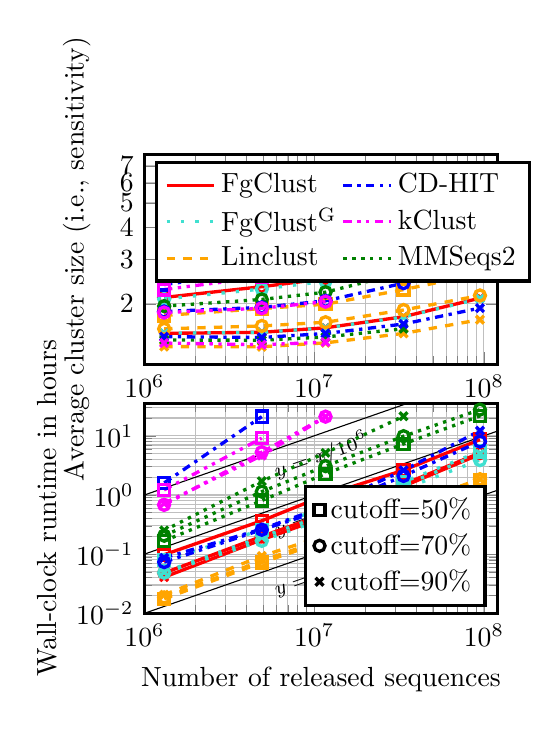
\begin{tikzpicture}
	\begin{groupplot}[group style={group size= 1 by 2,vertical sep=0.5cm},
	scaled x ticks=false,scaled y ticks=false,
	legend cell align={left},
	xmin=1e6,xmax=1.2e8,
	]
	
	\nextgroupplot[very thick,grid=both,
width=0.5\textwidth,height=0.35\textwidth,
mark options={solid},
ytick={1,2,3,4,5,6,7,8,9},log y ticks with fixed point,
ylabel={Average cluster size (i.e., sensitivity)},
legend columns=4,transpose legend,legend pos=north west,
%legend style={fill=none},
xmode=log,ymode=log,
legend entries={
	FgClust,FgClust\textsuperscript{G},
	Linclust,MMSeqs2,CD-HIT,kClust,
	%cutoff=50\%,cutoff=70\%,cutoff=90\%
},
]
\addlegendimage{,color=Red}
\addlegendimage{loosely dotted,color=Turquoise}
\addlegendimage{dashed,color=Orange}
\addlegendimage{dotted,color=Green}
\addlegendimage{dash dot,color=Blue}
\addlegendimage{dash dot dot,color=Magenta}

\addplot[color=Red,mark=square] coordinates {
(1306318,       1306318/422186)
(4910948,       4910948/1320766)
(11659891,      11659891/2872344)
(33613081,      33613081/6588205)
(94756963,      94756963/14317115)
}; %FgClust 50
\addplot[color=Red,mark=o] coordinates {
(1306318,       1306318/616047)
(4910948,       4910948/2100471)
(11659891,      11659891/4633711)
(33613081,      33613081/10996570)
(94756963,      94756963/24074495)
}; %FgClust 70
\addplot[color=Red,mark=x] coordinates {
(1306318,       1306318/853689)
(4910948,       4910948/3177750)
(11659891,      11659891/7244693)
(33613081,      33613081/18878368)
(94756963,      94756963/44982646)
}; %FgClust 90

\addplot[loosely dotted,color=Turquoise,mark=square] coordinates {
(1306318,       1306318/440536)
(4910948,       4910948/1397457)
(11659891,      11659891/3045461)
(33613081,      33613081/7030002)
(94756963,      94756963/15345559)
}; %FgClustG 50
\addplot[loosely dotted,color=Turquoise,mark=o] coordinates {
(1306318,       1306318/624838)
(4910948,       4910948/2145454)
(11659891,      11659891/4747777)
(33613081,      33613081/11334184)
(94756963,      94756963/24951918)
}; %FgClustG 70
\addplot[loosely dotted,color=Turquoise,mark=x] coordinates {
(1306318,       1306318/852268)
(4910948,       4910948/3178739)
(11659891,      11659891/7251378)
(33613081,      33613081/18927370)
(94756963,      94756963/45187681)
}; %FgClustG 90

\addplot[dashed,color=Orange,mark=square] coordinates {
	( 1306318,       1306318/       725566   )
	( 4910948,       4910948/       2562086  )
	(11659891,      11659891/       5847706  )
	(33613081,      33613081/       14766033 )
	(94756963,      94756963/       35983786 )
}; %Linclust 50
\addplot[dashed,color=Orange,mark=o] coordinates {
	( 1306318,       1306318/       819293    )
	( 4910948,       4910948/       3000298   )
	(11659891,      11659891/       6889416   )
	(33613081,      33613081/       17768118  )
	(94756963,      94756963/       43908412  )
}; %Linclust 70
\addplot[dashed,color=Orange,mark=x] coordinates {
	( 1306318,       1306318/       962908    )
	( 4910948,       4910948/       3625681   )
	(11659891,      11659891/       8306445   )
	(33613081,      33613081/       21974288  )
	(94756963,      94756963/       54672623  )
};

\addplot[dotted,color=Green,mark=square] coordinates {
	( 1306318,       1306318/       516052    )
	( 4910948,       4910948/       1670691   )
	(11659891,      11659891/       3611539   )
	(33613081,      33613081/       8247496 )
	(94756963,      94756963/       17763784        )
}; % mmseqs2 50
\addplot[dotted,color=Green,mark=o] coordinates {
	( 1306318,       1306318/       666575    )
	( 4910948,       4910948/       2358569   )
	(11659891,      11659891/       5244463   )
	(33613081,      33613081/       12622515        )
	(94756963,      94756963/       27872093        )
};
\addplot[dotted,color=Green,mark=x] coordinates {
	( 1306318,       1306318/       906871    )
	( 4910948,       4910948/       3415601   )
	(11659891,      11659891/       7874593   )
	(33613081,      33613081/       21060831        )
	%(94756963,      94756963/       77117011       ) % timeout
};

\addplot[dash dot,color=Blue,mark=square] coordinates {
	( 1303982 , 1303982 / 547396 )
	( 4908596 , 4908596 / 1818516 )
};
\addplot[dash dot,color=Blue,mark=o] coordinates {
	( 1303982 , 1303982 / 698797 )
	( 4908596 , 4908596 / 2532809 )
	( 11656604 , 11656604 / 5671408 )
	( 33606888 , 33606888 / 13921644 )
	( 94744006 , 94744006 / 31180026 )
};
\addplot[dash dot,color=Blue,mark=x] coordinates {
	( 1303982 , 1303982 / 878273 )
	( 4908596 , 4908596 / 3329592 )
	( 11656604 , 11656604 / 7627716 )
	( 33606888 , 33606888 / 20175146 )
	( 94744006 , 94744006 / 49205865 )	
};

\addplot[dash dot dot,color=Magenta,mark=square] coordinates {
	( 1303982 , 1303982 / 572347 )
	( 4908596 , 4908596 / 1924257 )
};
\addplot[dash dot dot,color=Magenta,mark=o] coordinates {
	( 1303982 , 1303982 / 705456 )
	( 4908596 , 4908596 / 2552951 )
	( 11656604 , 11656604 / 5713855 )
};
\addplot[dash dot dot,color=Magenta,mark=x] coordinates {
	( 1303982 , 1303982 / 930527 )
	( 4908596 , 4908596 / 3556609 )
	( 11656604 , 11656604 / 8250898 )
};

	\nextgroupplot[very thick, grid=both, width=0.5\textwidth, height=0.35\textwidth, mark options={solid},
xmode=log,ymode=log,
ymax=35,ymin=1e-2,
xlabel=Number of released sequences,
ylabel=Wall-clock runtime in hours,
legend columns=4,transpose legend,legend pos=south east,
legend entries={
	cutoff=50\%,cutoff=70\%,cutoff=90\%
},
]
\addlegendimage{only marks,mark=square}
\addlegendimage{only marks,mark=o}
\addlegendimage{only marks,mark=x}

\addplot[mark=none, black, thin, domain=5e5:2e8] {1e-8*x}
node[midway, below, sloped]{\scriptsize\(y=x/10^{8}\)};
\addplot[mark=none, black, thin, domain=5e5:2e8] {1e-7*x}
node[midway, below, sloped]{\scriptsize\(y=x/10^{7}\)};
\addplot[mark=none, black, thin, domain=5e5:2e8] {1e-6*x}
node[midway, below, sloped]{\scriptsize\(y=x/10^{6}\)};


\addplot[color=Red,mark=square] coordinates {
(1306318        ,       352.18/3600)
(4910948        ,       1320.00/3600)
(11659891       ,       3580.52/3600)
(33613081       ,       9433.11/3600)
(94756963       ,       30982.14/3600)
}; % FgClust 50
\addplot[color=Red,mark=o] coordinates {
(1306318        ,       172.90/3600)
(4910948        ,       717.59/3600)
(11659891       ,       1737.33/3600)
(33613081       ,       5468.15/3600)
(94756963       ,       18432.19/3600)
}; % FgClust 70
\addplot[color=Red,mark=x] coordinates {
(1306318        ,       146.88/3600)
(4910948        ,       631.00/3600)
(11659891       ,       1524.65/3600)
(33613081       ,       5059.81/3600)
(94756963       ,       17577.41/3600)
}; % FgClust 90

\addplot[loosely dotted,color=Turquoise,mark=square] coordinates {
(1306318        ,       283.35/3600)
(4910948        ,       925.34/3600)
(11659891       ,       2253.87/3600)
(33613081       ,       5983.02/3600)
(94756963       ,       19567.13/3600)
}; % FgClustG 50
\addplot[loosely dotted,color=Turquoise,mark=o] coordinates {
(1306318        ,       174.53/3600)
(4910948        ,       604.73/3600)
(11659891       ,       1462.27/3600)
(33613081       ,       4543.20/3600)
(94756963       ,       14003.26/3600)
}; % FgClustG 70
\addplot[loosely dotted,color=Turquoise,mark=x] coordinates {
(1306318        ,       178.76/3600)
(4910948        ,       701.40/3600)
(11659891       ,       1681.85/3600)
(33613081       ,       5248.21/3600)
(94756963       ,       17860.82/3600)
}; % FgClustG 90

\addplot[dashed,color=Orange,mark=square] coordinates {
	( 1306318,      63.24 / 3600)
	( 4910948,      259.20 / 3600)
	(11659891,      600.11 / 3600)
	(33613081,      1859.28 / 3600)
	(94756963,      6444.66 / 3600)
}; %linclust 50
\addplot[dashed,color=Orange,mark=o] coordinates {
	( 1306318,      66.58 / 3600)
	( 4910948,      278.11 / 3600)
	(11659891,      652.31 / 3600)
	(33613081,      2013.65 / 3600)
	(94756963,      6639.85 / 3600)
};
\addplot[dashed,color=Orange,mark=x] coordinates {
	( 1306318,      73.96 / 3600)
	( 4910948,      334.20 / 3600)
	(11659891,      744.64 / 3600)
	(33613081,      2270.75 / 3600)
	(94756963,      6698.25 / 3600)
};

\addplot[dotted,color=Green,mark=square] coordinates {
	( 1306318,      603.10 / 3600)
	( 4910948,      2898.67 / 3600)
	(11659891,      8230.45 / 3600)
	(33613081,      26272.73 / 3600)
	(94756963,      77837.47 / 3600)
};
\addplot[dotted,color=Green,mark=o] coordinates {
	( 1306318,      737.74 / 3600)
	( 4910948,      4098.65 / 3600)
	(11659891,      11068.39 / 3600)
	(33613081,      35445.09 / 3600)
	(94756963,      99781.83 / 3600)
};
\addplot[dotted,color=Green,mark=x] coordinates {
	( 1306318,      905.05 / 3600)
	( 4910948,      6154.68 / 3600)
	(11659891,      18524.44 / 3600)
	(33613081,      77145.61 / 3600)
	%(94756963,timeout)
};

\addplot[dash dot,color=Blue,mark=square] coordinates {
	( 1306318,      5766.21 / 3600)
	( 4910948,      75911.85 / 3600)
	%(11659891,timeout)
	%(33613081,timeout)
	%(94756963,timeout)
};
\addplot[dash dot,color=Blue,mark=o] coordinates {
	( 1306318,      264.31 / 3600)
	( 4910948,      929.93 / 3600)
	(11659891,      2062.60 / 3600)
	(33613081,      7563.33 / 3600)
	(94756963,      28834.18 / 3600)
};
\addplot[dash dot,color=Blue,mark=x] coordinates {
	( 1306318,      311.15 / 3600)
	( 4910948,      955.40 / 3600)
	(11659891,      2315.58 / 3600)
	(33613081,      9395.35 / 3600)
	(94756963,      43880.61 / 3600)
};

\addplot[dash dot dot,color=Magenta,mark=square] coordinates {
	( 1303982 , 4378.45 / 3600 )
	( 4908596 , 32820.26 / 3600 )
};
\addplot[dash dot dot,color=Magenta,mark=o] coordinates {
	( 1303982 , 2447.86 / 3600 )
	( 4908596 , 19014.50 / 3600 )
	( 11656604 , 75912.68 / 3600 )
};
\addplot[dash dot dot,color=Magenta,mark=x] coordinates {
	( 1303982 , 2597.88 / 3600 )
	( 4908596 , 16724.53 / 3600 )
	( 11656604 , 75284.21 / 3600 )
};
	
	\end{groupplot}
	\end{tikzpicture}
	
	\caption{
		%This figure shows the impact of database growth on sensitivity and runtime.
		UniProt released
		\SI{1306318}{},
		\SI{4910948}{}, 
		\SI{11659891}{}, 
		\SI{33613081}{}, and 
		\SI{94756963}{} 
		sequences into 
		UniRef100-2.0,
		UniRef100-12.0,
		UniRef100-2011-01, 
		UniRef100-2014-01, and
		UniRef100-2017-01
		in 
		July 2004,
		July 2017,
		January 2011,
		January 2014, and
		January 2017,
		respectively \citep{suzek2007uniref}.
		We ran each program on each release of the UniRef100 database with each similarity cutoff to generate each set of clusters.
		Cluster quality is not evaluated due to the lack of ground truth. 
		Each program times out after running for \SI{50}{} hours.
		FgClust\textsuperscript{G} is the special instance using greedy incremental update instead of click-aware all-versus-all search (\cref{subsec:clique-aware}).
		\label{fig:uniref}
	}
\end{figure}

In our evaluations, we made several exclusions.
First, we did not include UCLUST \citep{edgar2010search}, which can perform protein and nucleotide sequence clustering, because only the memory-limited 32-bit version of UCLUST is free and the software is not open source.
Second, we did not use gene ontology (GO).
GO terms with experimental evidence can be used for evaluating protein-function prediction \citep{radivojac2013large}.
However, very few sequences from the UniRef100-2017-01 dataset are annotated with experimental GO evidence \citep{suzek2014uniref}.
In fact, such annotated sequences generate approximately only 100 non-singleton clusters at 50\% sequence-similarity cutoff for clustering (data not shown).
Therefore, evaluation using experimental GO evidence may be too noisy to be reliable.
Thus, we omitted GO term similarity in our evaluation metrics.
Finally, we excluded the metrics of canonical specificity (i.e., either the percentage of clusters that are not corrupted or average consistency of each cluster).
The reason is that canonical specificity is not normalized against the input and is therefore not meaningful for measuring specificity (more detail in \cref{sec:appendix:canonical-specificity}).
Instead, we measured specificity using the average biological similarity between each input sequence and the representative centroid that covers the input sequence.
In this study, we used structural and/or functional similarity as a proxy of biological similarity.
We nonetheless included canonical specificity in \cref{sec:appendix:canonical-specificity}.

Before any evaluation, we shuffled the sequences in each biological database by using a random-number generator with the same seed.
Thus, our evaluation results were both deterministically and yet pseudo-randomly generated to be both reproducible and unaffected by the order of sequences in database (i.e., bias-free).
Moreover, all evaluations are done on a ``CentOS release 6.6'' server that runs on ``Intel(R) Xeon(R) CPU E5-2660 0 @ 2.20GHz'' with 16 cores and 32 threads.

\subsection{Evaluation on five releases of protein sequences in UniRef100}

We evaluated the sensitivity, scalability, and runtime of FgClust using several releases of a gold-standard protein sequence database.
We downloaded the five releases of UniRef100 \citep{suzek2007uniref} listed in \cref{fig:uniref}.
From each release of UniRef100, we extracted the protein sequences.
From these extracted sequences, each sequence-clustering algorithm was used to generate a set of clusters.
The number of clusters produced by each algorithm and the runtime of each algorithm were recorded (\cref{fig:uniref}).

A more sensitive clustering algorithm generates fewer clusters of larger average cluster size.
FgClust generates the fewest clusters with the largest average cluster size (\cref{fig:uniref}), indicating that FgClust is the most sensitive method.
Moreover, FgClust is always faster than MMSeqs2, CD-HIT, and kClust (\cref{fig:uniref}).
FgClust, however, is slower but significantly more sensitive than Linclust  (\cref{fig:uniref}).
In fact, Linclust generates approximately 70\% and 150\% more clusters than FgClust at 50\% similarity cutoff on UniRef100-2.0 and UniRef100-2017-01, respectively (\cref{fig:uniref}).
This indicates that the sensitivity of Linclust significantly decreases as the size of the input database increases. 
Overall, our results suggest that, among the algorithms evaluated, only FgClust can scale to future releases of UniRef100 in terms of both sensitivity and runtime.
The improved sensitivity of FgClust on UniRef100 
results from the use of 
%the Murphy10 reduced alphabet (data not shown) and 
clique-aware all-versus-all search, especially at low sequence-similarity cutoffs (e.g., 50\%).
In fact, compared with clique-aware all-versus-all search presented in \cref{subsec:clique-aware}, greedy incremental update produces up to more than 7.0\% more clusters and only reduces runtime by at most 35\% (\cref{fig:uniref}).
The runtime improvement of FgClust on UniRef100 can be explained by 
the use of 
%search up to a maximum number of consecutive failed attempts and 
%a limited number of centroid-sequence candidates per indexed k-mer group instead of an unlimited such number (data not shown) and 
edit-similarity instead of alignment statistics as cutoff \citep{vsovsic2017edlib}.
%In fact, the special instance of FgClust using greedy incremental update can even match the runtime of Linclust (\cref{fig:uniref}).
FgClust and Linclust seem to be characterized by sightly super-linear runtime in \cref{fig:uniref} because the average protein length slightly increases in each newer release. Therefore, if the distribution of sequence lengths remain unchanged in different releases, then FgClust and Linclust would be indeed characterized by linear runtime.

Linclust
selects only one centre sequence per k-mer, 
selects certain k-mers in each input sequence, 
and then tries to cluster the input sequence with any of the centre sequences corresponding to these k-mers.
Input sequences that cannot be clustered with any such centre sequence remain as singletons.
Thus, Linclust is not sufficiently sensitive.
As suggested by \citet{steinegger2017linclust},
we increased the number of k-mers selected in each input sequence to 80 in an attempt to improve the sensitivity of Linclust.
However, this attempt resulted in virtually the same average cluster sizes for Linclust to the point that \cref{fig:uniref} would remain visually unchanged. Hence, the sensitivity of Linclust remains practically unchanged.
FgClust is significantly faster than MMSeqs2 especially at any high sequence similarity cutoff.
FgClust is significantly more scalable than CD-HIT and kClust. 
In fact, CD-HIT is characterized by slow and super-linear runtime, particularly at 50\% sequence-identity cutoff.
CD-HIT compares each query input sequence with each target input sequence that shares at least one k-mer with the query input sequence.
kClust compares each query input sequence with each target input sequence that has at least one k-mer similar (i.e., in terms of alignment score) to any k-mer in the query input sequence.
The probability that two sequences possess similar k-mers by random chance is relatively constant, and therefore does not depend on the number of input sequences.
Consequently, as the number of input sequences increases linearly, the number of pairwise comparisons triggered by random chance increases quadratically.
Thus, the runtime of CD-HIT and kClust is asymptotically quadratic with respect to input size.
The use of longer k-mers significantly reduces the probability that two sequences share the same longer k-mer by random chance.
Therefore, the use of longer k-mers implies that more input sequences are required to trigger the quadratic runtime of CD-HIT.
Indeed, the runtime of CD-HIT with five million sequences as input is roughly quadratic at 50\% sequence-identity cutoff but still roughly linear at 70\% or more sequence-identity cutoff (\cref{fig:uniref}).
FgClust and MMSeqs2 use longer k-mers for a larger number of input sequences to maintain a linear expected runtime with respect to the number of input sequences.

Currently, each month, UniProt uses CD-HIT to cluster UniRef100 at 90\% sequence-identity cutoff into UniRef90, and then a distributed version of CD-HIT to cluster UniRef90 at 50\% sequence-identity cutoff into UniRef50 \citep{suzek2014uniref}.
Because of the quadratic runtime of CD-HIT at 50\% sequence-identity, CD-HIT will likely be unable to cope with the monthly release of UniRef50 in the future.
Our results suggest that FgClust is the best candidate for generating UniRef50 reasonably fast, not only because of significantly better runtime but also because the resulting UniRef50 would contain fewer representative sequences.

\subsection{Evaluation on protein structures in PDB}

\begin{table}%[!htbp]
	\centering
	\caption[]{
		The sequences of \SI{49686} monomeric proteins in PDB deposited exclusively before January 2\textsuperscript{nd} 2017 are given as input to each program \citep{berman2006protein}. 
		Each program is run with each similarity cutoff to generate each set of clusters.
		The template-modeling (TM) score between each representative cluster centroid and each sequence covered by the centroid is tabulated. A centroid trivially covers itself with a TM score of 1.
		If the TM score is at most 0.5, then the centroid and covered sequence are usually significantly different in protein structure
		\citep{xu2010significant}.
		%The wall-clock runtime of each program is too short to measure scalability.
		The special instance of FgClust using greedy incremental update and the default instance of FgClust using click-aware all-versus-all search produced similar results on this dataset. 
		Hence, results produced by the special instance are not presented.
	}
	\begin{tabular}{l c c c c c c}
		\toprule
		Program & similarity  & number of & 
		\multicolumn{4}{c}{TM scores} \\
		& cutoff      & clusters  &
		~\(\le\) 0.3~ & ~\(\le\) 0.4~ & ~\(\le\) 0.5~
		& ~\(\le\) 0.6~ \\%& ~\(\le\) 0.7~ & ~\(\le\) 0.8~ & ~\(\le\) 0.9~ \\
		\midrule
		
		%FgClust   & 50\% & 14784 &  88 & 248 & {\bfseries 547} & 1149 \\ %& 2150 & 3855 & 8227 \\
		FgClust   & 50\% & 14391 & 86 & 235 & {\bfseries 538} & 1187 \\
		Linclust  & 50\% & 17381 & 166 & 390 & 708 & 1160 \\ %& 1854 & 3010 & 5831 \\
		MMSeqs2   & 50\% & 15160 & 226 & 515 & 938 & 1790 \\ %& 2862 & 4445 & 8651 \\
		CD-HIT    & 50\% & 15658 & 266 & 574 & 981 & 1697 \\ %& 2628 & 3961 & 7305 \\
		kClust    & 50\% & 16108 & 181 & 423 & 809 & 1404 \\ %& 2179 & 3505 & 6884 \\ 
		\noalign{\vskip 2mm} 
		%FgClust   & 70\% & 17538 &  47 & 141 & {\bfseries 340} & 676 \\ %& 1285 & 2311 & 4387 \\
		FgClust   & 70\% & 17562 &  46 & 139 & {\bfseries 328}  & 659 \\
		Linclust  & 70\% & 18207 & 174 & 402 & 674 & 1083 \\ %& 1702 & 2709 & 4912 \\
		MMSeqs2   & 70\% & 17158 & 236 & 506 & 826 & 1355 \\ %& 2107 & 3209 & 5600 \\
		CD-HIT    & 70\% & 17610 & 242 & 464 & 751 & 1265 \\ %& 1956 & 2998 & 5308 \\
		kClust    & 70\% & 17682 & 187 & 405 & 695 & 1188 \\ %& 1811 & 2837 & 5244 \\
		\noalign{\vskip 2mm} 
		%FgClust   & 90\% & 19993 &  17 & 66  & {\bfseries 169} & 346 \\ %& 736  & 1359 & 2975 \\
		FgClust   & 90\% & 20030 & 17  & 57  & {\bfseries 161}  & 335 \\
		Linclust  & 90\% & 19552 & 125 & 284 & 507 & 872  \\ %& 1378 & 2149 & 3834 \\
		MMSeqs2   & 90\% & 18783 & 219 & 426 & 734 & 1143 \\ %& 1810 & 2717 & 4669 \\
		CD-HIT    & 90\% & 19124 & 189 & 364 & 586 & 940  \\ %& 1485 & 2300 & 4041 \\
		kClust    & 90\% & 19707 & 141 & 315 & 513 & 848  \\ %& 1306 & 2128 & 3800 \\
		\bottomrule
	\end{tabular}
	\label{table:pdb}
\end{table}
%\footnotetext{The special instance of FgClust using greedy incremental update and the default instance of FgClust using click-aware all-versus-all search produced similar results on this dataset. 
%	Hence, results produced by the special instance are not presented.}

We evaluated the sensitivity and specificity of FgClust by using three-dimensional alignments of experimentally determined protein structures.
We downloaded all monomeric proteins with experimentally determined structures deposited into PDB exclusively before January 2\textsuperscript{nd} 2017 \citep{berman2006protein}.
The sequence of each protein is extracted.
If an extracted sequence has at least 11 non-ambiguous amino acids and at least 90\% amino acids of the extracted sequence are non-ambiguous, then the extracted sequence is kept.
From these kept sequences, each sequence-clustering algorithm was used to generate a set of clusters.
Within each cluster, the template-modeling (TM) score between the representative sequence and each represented sequence is computed by TM-Align \citep{zhang2005tm}.
A lower TM score means a lower specificity achieved by a clustering algorithm.
FgClust generates the fewest number of sequences with low TM scores (i.e., at most 0.5) to their centroids (\cref{table:pdb}).
Usually, two proteins are in the same fold if and only if these two proteins share a TM-score of more than 0.5 \citep{xu2010significant}, where a protein fold is defined by the arrangement of the secondary structure elements relative to each other in space.
As a result, FgClust is significantly more specific than other algorithms in terms of experimentally determined protein structures.
Furthermore, FgClust at 50\% similarity cutoff generates the fewest clusters with the highest average cluster size.
Therefore, FgClust is significantly more specific and sensitive than other algorithms in terms of protein structural similarity.
%The better specificity and sensitivity of FgClust on PDB structures are attributed to the use of Murphy10 to reduce amino-acid alphabet and 25 residues to normalize edit-similarity, respectively (data not shown).

\subsection{Evaluation on protein families in Pfam}

\begin{figure}%[!htbp]
	\centering
	
	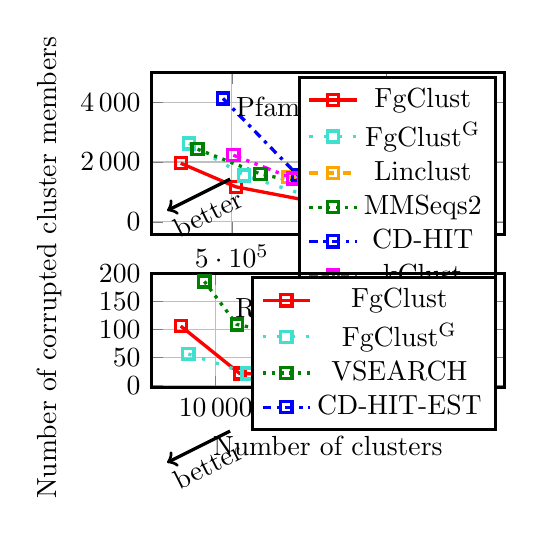
\begin{tikzpicture}
	\begin{groupplot}[group style={group size= 1 by 2,vertical sep=0.5cm}]
	\nextgroupplot[very thick,grid=both,
	mark options={solid},
	width=0.5\textwidth,
	height=0.3\textwidth,
	ymax=5000,
	scaled x ticks=false,
	scaled y ticks=false,
	title style={xshift=-5ex,yshift=-6ex},
	title={Pfam},
	%legend columns=2,legend pos=north east,
	]
	\addplot[color=Red,mark=square] coordinates {
		(335000,1959)
		(512685,1171)
		(763066,675)
		(1071036,287)
		(1282437,77)
	};
	\addlegendentry{FgClust}
	\addplot[loosely dotted,color=Turquoise,mark=square] coordinates {
		(361612,2621)
		(539571,1552)
		(783414,744)
		(1078159,294)
		(1282380,77)
	};
	\addlegendentry{FgClust\textsuperscript{G}}
	\addplot[dashed,color=Orange,mark=square] coordinates {
		(682422, 1501)
		(806160, 1111)
		(982978, 749)
		(1199664, 445)
		(1281061, 193)
	};
	\addlegendentry{Linclust}
	\addplot[dotted,color=Green,mark=square] coordinates {
		(389286, 2429)
		(592144, 1602)
		(843097, 1037)
		(1128443, 561)
		(1253416, 294)
	};
	\addlegendentry{MMSeqs2}
	\addplot[dash dot,color=Blue,mark=square] coordinates {
		(471396, 4126)
		(713570, 1549)
		(976870, 705)
		(1252062, 342)
		(1284604, 139)
	};
	\addlegendentry{CD-HIT}
	\addplot[dash dot dot,color=Magenta,mark=square] coordinates {
		(504834,2230)
		(697636,1452)
		(947935,804)
		(1221908,379)
		(1283087,149)
	};
	\addlegendentry{kClust}
	
	\nextgroupplot[very thick,grid=both,
	mark options={solid},
	width=0.5\textwidth,
	height=0.25\textwidth,
	ymax=200,%ymode=log,ymax=1000,
	xlabel=Number of clusters,% (Rfam),
	scaled x ticks=false,
	scaled y ticks=false,
	title style={xshift=-5ex,yshift=-6ex},
	title={Rfam},
	]
	
	\addplot[color=Red,mark=square] coordinates {
		(6704,106)
		(12261,21)
		(21164,18)
		(34266,14)
	};
	\addlegendentry{FgClust}
	\addplot[loosely dotted,color=Turquoise,mark=square] coordinates {
		(7419,56)
		(13005,21)
		(21762,18)
		(34412,14)
	};
	\addlegendentry{FgClust\textsuperscript{G}}
	
	\addplot[dotted,color=Green,mark=square] coordinates {
		%(7509, 1958)
		(8929, 186)
		(11978, 109)
		(18085, 84)
		(27963, 67)
	};
	\addlegendentry{VSEARCH}
	\addplot[dash dot,color=Blue,mark=square] coordinates {
		(15074, 100)
		(26608, 44)
	};
	\addlegendentry{CD-HIT-EST}
	\end{groupplot}
	\path (current bounding box.west)-- node[anchor=south,rotate=90] {Number of corrupted cluster members} (current bounding box.west);
	\draw[->,very thick](1,0.7)--(0.2,0.3)node
	[midway,below,sloped]{better};
	\draw[->,very thick](1,-2.5)--(0.2,-2.9)node
	[midway,below,sloped]{better};
	\end{tikzpicture}
	
	\caption{Results of clustering Pfam-A-seed release 31.0 \citep{finn2016pfam} and Rfam-seed release 12.3 \citep{nawrocki2014rfam}.
		On each plotted curve, the five marks from left to right correspond to the five sequence-similarity cutoffs of 50\% (only for Pfam), 60\%, 70\%, 80\%, and 90\%, respectively.
		CD-HIT-EST does not run with any sequence-similarity cutoff of less than 80\%.
		A cluster member is corrupted if and only if the member belongs to a Pfam or Rfam family that the representative of the cluster does not belong to.
		%The wall-clock runtime of each program is too short to measure scalability.
		FgClust\textsuperscript{G} is the special instance using greedy incremental update instead of click-aware all-versus-all search (\cref{subsec:clique-aware}).
		\label{fig:pfam}
		\label{fig:rfam}
	}
\end{figure}

Pfam offers a benchmark for the classification of functional protein domains \citep{finn2016pfam}.
For this evaluation, we applied each clustering algorithm on
the manually checked seed A dataset from Pfam release 31.0 \citep{finn2016pfam}.
We assessed the quality of the clusters in terms of 
the number of corrupted sequences contained by a cluster.
We regarded a sequence, or a member of a cluster, to be corrupted if it belongs to a Pfam family that the representative of the cluster does not belong to.
A more sensitive clustering algorithm generates fewer clusters, whereas a more specific clustering algorithm generates fewer corrupted cluster members.
As previously mentioned, 
the number of corrupted clusters (a corrupted cluster contains sequences belonging to different families) is not normalized against the input and is therefore not meaningful for measuring specificity.
However, the number of corrupted clusters can reveal the characteristics of different clustering algorithms and is therefore still shown in \cref{fig:pfam-appendix}.
We found that FgClust generates much fewer clusters given the same number of corrupted cluster members and much fewer corrupted cluster members given the same number of clusters (\cref{fig:pfam}).
The result shows that FgClust is significantly more sensitive at the same specificity and significantly more specific at the same sensitivity.
Therefore, FgClust achieves the best sensitivity-specificity trade-off.
The use of clique-aware all-versus-all search instead of greedy incremental update significantly improved both the sensitivity and specificity of FgClust on Pfam-A-seed (\cref{fig:pfam}).
%The sensitivity of FgClust on Pfam-A-seed is mostly improved by the use of Murphy10 reduced alphabet (data not shown) and the use of clique-aware all-versus-all search instead of greedy incremental update (\cref{fig:pfam}).
%The specificity of FgClust on Pfam-A-seed is mostly improved by the use of 25 residues to normalized edit-similarity (data not shown) and the use of clique-aware all-versus-all search instead of greedy incremental update (\cref{fig:pfam}). 
In fact, compared with clique-aware all-versus-all search, greedy incremental update produces up to 8.0\% more clusters and 34\% more corrupted cluster members (\cref{fig:pfam}).
%We tried shortening the length of indexed long words and increasing the number of attempts (parameter \(W\) in \cref{alg:fgclust}) at the same time.
%However, none of the combinations of such approaches to increase sensitivity can result in more than 8\% reduction in the number of clusters without at least one order of magnitude increase in runtime (data not shown). 
Similar to using clique-aware all-versus-all search, increasing the e-value (or equivalently, reducing the length) of indexed k-mers also improves sensitivity.
However, using clique-aware all-versus-all search results in better sensitivity-runtime trade-off than increasing the e-value of indexed k-mers (\cref{fig:pfam-sensitivity-runtime}).
In other words, using clique-aware all-versus-all search can result in the same sensitivity with less runtime (and the same runtime with more sensitivity) than reducing the length of indexed k-mers.
Therefore, clique-aware all-versus-all search significantly improves sensitivity in a unique way.

At low sequence-similarity cutoffs (e.g., 50\%),
CD-HIT has the worst sensitivity-specificity trade-off, presumably because inferring biological similarity from a low sequence identity is highly error-prone.
FgClust normalizes edit-similarity with respect to sequence length.
Linclust, MMSeqs2, and kClust use e-value in addition to sequence identity.
As a result, FgClust, Linclust, MMSeqs2, and kClust do not suffer from a drop in sensitivity-specificity trade-off at a low sequence similarity.
Linclust, MMSeqs2, and kClust use iterative, profile-based clustering strategy and can thus merge similar clusters into one single cluster.
A false-positive merging step corrupts only one cluster, but it can corrupt multiple cluster members.
Thus, Linclust, MMSeqs2, and kClust generate high numbers of corrupted cluster members compared with the numbers of corrupted clusters (\cref{fig:pfam,fig:pfam-appendix}).



\subsection{Evaluation on RNA families in Rfam}

Rfam provides a gold-standard benchmark for the classification of non-coding RNA sequences \citep{nawrocki2014rfam}.
In this study, we utilized the manually checked seed dataset from Rfam release 12.3 \citep{nawrocki2014rfam}.
Evaluation metrics for Pfam and Rfam are similar.
In our experiments, we found that FgClust generates much fewer clusters given the same number of corrupted cluster members and much fewer corrupted cluster members given the same number of clusters (\cref{fig:rfam}).
This result indicates that FgClust achieves the best overall sensitivity-specificity trade-off.
%The sensitivity and specificity of FgClust on Rfam-seed are mostly improved by the use of edit-similarity instead of sequence identity as the cutoff (data not shown).
%The specificity of FgClust on Rfam-seed is also improved by the use of 25 residues to normalized edit-similarity (data not shown).









%\section{Discussion}





%%%%%%%%%%%%%%%%%%%%%%%%%%%%%%%%%%%%%%%%%%%%%%%%%%%%%%%%%%%%%%%%%%%%%%%%%%%%%%%%%%%%%
%
%     please remove the " % " symbol from \centerline{\includegraphics{fig01.eps}}
%     as it may ignore the figures.
%
%%%%%%%%%%%%%%%%%%%%%%%%%%%%%%%%%%%%%%%%%%%%%%%%%%%%%%%%%%%%%%%%%%%%%%%%%%%%%%%%%%%%%%









\section{Conclusion}

We developed FgClust, a novel algorithm for clustering biological sequences.
FgClust is more sensitive, more specific, and faster than other state-of-the-art clustering algorithms, except that Linclust is approximately three times faster but also generates up to more than 150\% more clusters than FgClust.
We observed that greedy incremental update may not select the optimal centroid during each incremental update.
Accordingly, FgClust detects a sufficient number of sequence pairs such that, in each pair, the first can represent the second.
Then, FgClust uses greedy set cover to cluster all sequences based on such pairings.
We observed that an indexed k-mer can be non-informative for some sequences and yet informative for some other sequences.
Accordingly, FgClust imposes a reasonable limit on the number of centroid-sequence candidates for each indexed k-mer group.
%We observed that there are too many short words in a typical biological sequence.
%Accordingly, FgClust uses min-hash values instead of short words as filter.
We observed that sequence identity is not sufficiently correlated with biological similarity and requires the time-consuming computation of alignment.
Accordingly, FgClust uses edit-similarity instead of sequence identity.
%Edit-similarity is defined as one minus the following: 
%	number of single-character edits to change a member sequence into a substring of the centroid sequence, divided by the length of the member sequence.

FgClust generates clusters of the highest quality. 
Consequently, FgClust reduces manual-curation efforts and errors in the downstream analysis of clusters.
For example, sequences in the same cluster can be assumed to be homologous to each other for homology modeling.
Errors in homology modeling are reduced by the use of FgClust.
This reduction in errors results in less manual examination of the errors and improves the prediction of structures and functions \citep{nayeem2006comparative}.
Moreover, FgClust is fast and scalable.
FgClust will be able to handle the large volume of sequences released by UniProt and metagenomic studies.

In the future, we will construct a Hidden Markov Model (HMM) for each cluster generated by FgClust and evaluate the quality of such HMMs. These HMMs should be able to detect most distant homology to enable deeper clustering \citep{steinegger2017mmseqs2}.
Moreover, we will apply the techniques used in FgClust to other problems, such as metagenomics-sequence classification and chimera detection.%, and detection of conserved protein domains.

%\section*{Acknowledgements}
%Text Text Text Text Text Text  Text Text.  \citealp{Boffelli03} might want to know about  text
%text text text\vspace*{-12pt}

\section*{Funding}

This work has been supported by the... Text Text  Text Text.\vspace*{-12pt}

%\bibliographystyle{natbib}
%\bibliographystyle{achemnat}
%\bibliographystyle{plainnat}
%\bibliographystyle{abbrv}
%\bibliographystyle{bioinformatics}
%
%\bibliographystyle{plain}
%
%\bibliography{Document}

\bibliographystyle{natbib}

\bibliography{mybib}

\clearpage{}

\section*{Supplementary information}


\subsection{Canonical specificity is not normalized against input}
\label{sec:appendix:canonical-specificity}
Canonical clustering sensitivity is the average number of sequences in each cluster.
Canonical clustering specificity is either the percentage of clusters that are not corrupted \citep{hauser2013kclust} or the average consistency of each cluster \citep{hauser2016mmseqs,steinegger2017mmseqs2,steinegger2017linclust}.
By definition, all singletons (i.e., clusters that contain only one sequence per cluster) are not corrupted and are characterized by the highest consistency.
However, if a large number of input sequences are clustered into one large cluster and a large number of singletons, then the resulting clusters achieve both high canonical sensitivity and high canonical specificity.
For example, one million sequences can be partitioned into one thousand clusters such that one cluster contains \SI{999001} sequences and the other \SI{999} clusters contain one sequence each.
In this case, 
the canonical sensitivity is high because only one thousand clusters are generated out of one million sequences, 
and the canonical specificity is high because only the cluster containing \SI{999001} sequences is corrupted and/or not characterized by the highest consistency.
As a result, canonical specificity is not normalized against the input and is therefore not meaningful for measuring specificity.

\clearpage{}

\begin{table}%[!htbp]
	\centering
	\caption{
		Extension of \cref{table:pdb} to include canonical specificity.
		In this case, canonical specificity is measured by intra-cluster template-modeling (TM) score.
		%The sequences of \SI{49686} monomeric proteins in PDB deposited exclusively before January 2\textsuperscript{nd} 2017 are given as input to each program \citep{berman2006protein}. 
		%Each program is run with each similarity cutoff to generate each set of clusters.
		The intra-cluster TM score of a cluster is the lowest TM score between the representative sequence in the cluster as template and each represented sequence in the cluster.
		For each set of clusters, the number of sequences characterized by intra-cluster TM scores inclusively below each threshold is tabulated.
		%A cluster with an intra-cluster TM-score of at most 0.5 contains at least one outlier in terms of three-dimensional structure and thus is of bad quality 
		%If the TM score is at most 0.5, then the centroid and covered sequence are significantly different in protein structure
		%\citep{xu2010significant}.
		%FgClust generates the least number of bad-quality clusters.
		%The wall-clock runtime of each program is too short to measure scalability.
	}
	\begin{tabular}{l c c c c c c c c}
		\toprule
		Program & similarity & 
		\multicolumn{5}{c}{intra-cluster TM scores} \\
		& cutoff (\%)     & ~\(\le\)0.2~ &
		~\(\le\)0.3~ & ~\(\le\)0.4~ & ~\(\le\)0.5~ 
		& ~\(\le\)0.6~ & ~\(\le\)0.7~ %& ~\(\le\)0.8~ & ~\(\le\)0.9~ & ~\(\le\)1~ \\
		\\
		\midrule
		
		FgClust & 50 & 4 & 58 & 141 & 290 & 582 & 1061 \\
		
		Linclust & 50 & 28 & 108 & 232 & 380 & 617 &  975 \\ % & 1490 \\ %& 2298 & 17381 \\
		MMSeqs2  & 50 & 32 & 132 & 263 & 424 & 701 & 1113 \\ % & 1654 \\ %& 2499 & 15160 \\
		CD-HIT   & 50 & 44 & 139 & 281 & 438 & 695 & 1114 \\ % & 1634 \\ %& 2440 & 15658 \\
		kClust   & 50 & 29 & 114 & 250 & 397 & 628 & 1017 \\ % & 1530 \\ %& 2351 & 16108 \\
		\noalign{\vskip 2mm} 

		FgClust & 70 & 3 & 28 & 82 & 180 & 376 & 712 \\
		Linclust & 70 & 28 & 110 & 225 & 360 & 577 & 907  \\ % & 1382 \\ %& & 2123 & 18207 \\
		MMSeqs2  & 70 & 32 & 127 & 251 & 391 & 629 & 995  \\ % & 1475 \\ %& & 2236 & 17158 \\
		CD-HIT   & 70 & 41 & 129 & 247 & 380 & 592 & 923  \\ % & 1398 \\ %& & 2121 & 17610 \\
		kClust   & 70 & 29 & 113 & 228 & 366 & 560 & 881  \\ % & 1335 \\ %& & 2063 & 17682 \\
		\noalign{\vskip 2mm} 
		
		FgClust & 90 & 2 & 9 & 31 & 90 & 196 & 397 \\
		Linclust & 90 & 20 &  85 & 177 & 302 & 479 & 763  \\ % & 1175 \\ %& & 1889 & 19552 \\
		MMSeqs2  & 90 & 35 & 111 & 217 & 358 & 549 & 826  \\ % & 1252 \\ %& & 1962 & 18783 \\
		CD-HIT   & 90 & 33 & 115 & 226 & 344 & 517 & 782  \\ % & 1171 \\ %& & 1852 & 19124 \\
		kClust   & 90 & 28 &  97 & 194 & 307 & 471 & 725  \\ % & 1083 \\ %& & 1732 & 19707 \\
		
		\bottomrule
	\end{tabular}
	\label{table:pdb-appendix}
\end{table}



\begin{figure}%[!htbp]
	\centering
	
		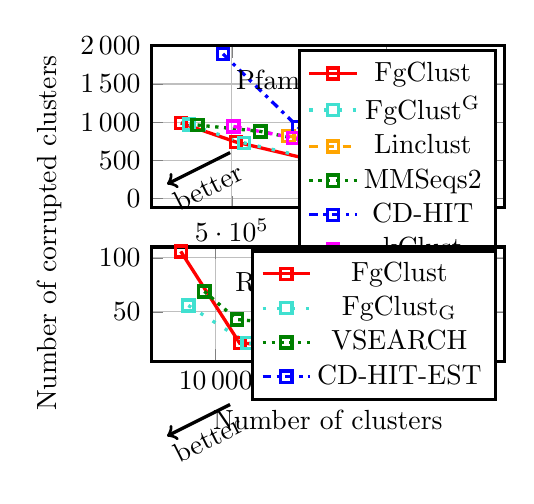
\begin{tikzpicture}
		\begin{groupplot}[group style={group size= 1 by 2,vertical sep=0.5cm}]
		\nextgroupplot[very thick,grid=both,
		mark options={solid},
		width=0.5\textwidth,
		height=0.3\textwidth,
		ymax=2000,
		scaled x ticks=false,
		scaled y ticks=false,
		title style={xshift=-5ex,yshift=-6ex},
		title={Pfam},
		]
		\addplot[color=Red,mark=square] coordinates {
(335000,989)
(512685,740)
(763066,500)
(1071036,247)
(1282437,71)
		};
		\addlegendentry{FgClust}
		\addplot[loosely dotted,color=Turquoise,mark=square] coordinates {
(361612,968)
(539571,728)
(783414,500)
(1078159,241)
(1282380,71)
		};
		\addlegendentry{FgClust\textsuperscript{G}}
		\addplot[dashed,color=Orange,mark=square] coordinates {	
			(682422, 819)
			(806160, 726)
			(982978, 572)
			(1199664, 401)
			(1281061, 188)
		};
		\addlegendentry{Linclust}
		\addplot[dotted,color=Green,mark=square] coordinates {
			(389286, 962)
			(592144, 878)
			(843097, 670)
			(1128443, 462)
			(1253416, 260)
		};
		\addlegendentry{MMSeqs2}
		\addplot[dash dot,color=Blue,mark=square] coordinates {
			(471396, 1894)
			(713570, 936)
			(976870, 558)
			(1252062, 317)
			(1284604, 135)
		};
		\addlegendentry{CD-HIT}
		\addplot[dash dot dot,color=Magenta,mark=square] coordinates {
			(504834,944)
			(697636,794)
			(947935,578)
			(1221908,331)
			(1283087,141)
		};
		\addlegendentry{kClust}
		%\draw[->,very thick](2,1.5)--(0.5,0.5)node
		%[midway,below,sloped]{better};
		\nextgroupplot[very thick,grid=both,
		mark options={solid},
		width=0.5\textwidth,
		height=0.25\textwidth,
		ymax=110,%ymode=log,
		xlabel=Number of clusters,% (Rfam),
		scaled x ticks=false,
		scaled y ticks=false,
		title style={xshift=-5ex,yshift=-6ex},
		title={Rfam},
		]
		\addplot[color=Red,mark=square] coordinates {
(6704,106)
(12261,21)
(21164,18)
(34266,14)
		};
		\addlegendentry{FgClust}
		\addplot[loosely dotted,color=Turquoise,mark=square] coordinates {
(7419,56)
(13005,21)
(21762,18)
(34412,14)
		};
		\addlegendentry{FgClust\textsubscript{G}}
		\addplot[dotted,color=Green,mark=square] coordinates {
			%(7509, 126)
			(8929, 69)
			(11978, 43)
			(18085, 38)
			(27963, 46)
		};
		\addlegendentry{VSEARCH}
		\addplot[dash dot,color=Blue,mark=square] coordinates {
			(15074, 36)
			(26608, 21)
		};
		\addlegendentry{CD-HIT-EST}
		%\draw[->,very thick](10,10)--(-10,-10)node
		%[midway,below,sloped]{better};
		\end{groupplot}
		\path (current bounding box.west)-- node[anchor=south,rotate=90] {Number of corrupted clusters} (current bounding box.west);
		\draw[->,very thick](1,0.7)--(0.2,0.3)node
		[midway,below,sloped]{better};
		\draw[->,very thick](1,-2.5)--(0.2,-2.9)node
		[midway,below,sloped]{better};
		\end{tikzpicture}
	
	\caption{
		Extension of \cref{fig:pfam} to include canonical specificity.
		In this case, canonical specificity is high if and only the number of corrupted clusters is low.
		A cluster is corrupted if and only if at least one member in the cluster belongs to a Pfam or Rfam family that the representative of the cluster does not belong to.
		\label{fig:pfam-appendix}
	}
\end{figure}




\begin{figure}
\begin{center}
\begin{tikzpicture}
\begin{axis}[very thick,
mark options={solid},
width=0.5\textwidth,
height=0.1\textwidth,
%legend style={draw=white!15!black,legend cell align=left}
legend style={at={(0.5,0.5)},anchor=south},
legend cell align=left,
xmin=1,ymin=1,xmax=2,ymax=2,
hide axis,
]
%\addplot[color=Red,mark=square] coordinates {(0,0)};
\addlegendimage{dotted,Red,mark=square}
\addlegendentry{\(E \in \{160,80,40,20,10\}, T=1\)};
\addlegendimage{dotted,Orange,mark=o}
\addlegendentry{\(T \in \{16,8,4,2,1\}, E=10\)};
\addlegendimage{dotted,Green,mark=x}
\addlegendentry{\(W \in \{10^4,10^3,10^2,10^1,10^0\}, E=0.01\)};
\addlegendimage{dotted,Turquoise,mark=diamond}
\addlegendentry{\(W \in \{10^4,10^3,10^2,10^1,10^0\}, E=1\)};
\addlegendimage{dotted,Blue,mark=+}
\addlegendentry{\(W \in \{10^4,10^3,10^2,10^1,10^0\}, E=100\)};
\end{axis}
\end{tikzpicture}
\end{center}
%\vspace{0.5cm}
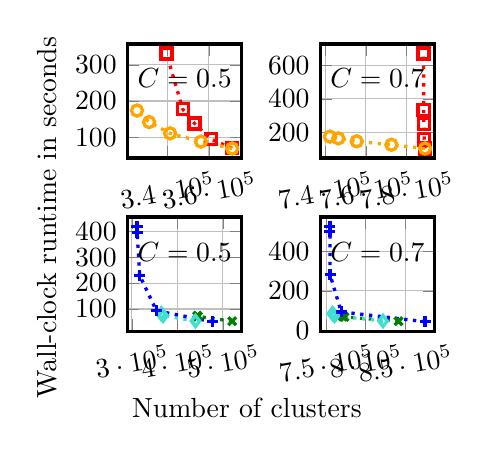
\begin{tikzpicture}
\begin{groupplot}[group style={group size= 2 by 2,vertical sep=0.75cm},
]

\nextgroupplot[very thick,grid=both,
mark options={solid},
width=0.25\textwidth,
height=0.25\textwidth,
%x tick label style={/pgf/number format/sci},
scaled x ticks=false,
x tick label style={rotate=10},
title style={yshift=-6ex},
title={\(C=0.5\)},
]
\addplot[dotted,color=Red,mark=square,] coordinates {
	(371131, 69.19)
	(360885, 94.81)
	(353156, 137.74)
	(347474, 177.32)
	(339690, 331.58)
};
\addplot[dotted,color=Orange,mark=o,] coordinates {
	(371131, 68.54)
	(356224, 87.57)
	(341412, 110.41)
	(331380, 141.59)
	(325601, 173.66)
};


\nextgroupplot[very thick,grid=both,
mark options={solid},
width=0.25\textwidth,
height=0.25\textwidth,
scaled x ticks=false,
x tick label style={rotate=10},
title style={yshift=-6ex},
title={\(C=0.7\)},
]
\addplot[dotted,color=Red,mark=square,] coordinates {
	( 789127 ,      102.23 )
	( 788726 ,      157.18 )
	( 788531 ,      247.85 )
	( 788457 ,      332.09 )
	( 788379 ,      671.89 )
};
\addplot[dotted,color=Orange,mark=o,] coordinates {
	( 789127 ,      102.32 )
	( 772570 ,      124.68 )
	( 755486 ,      145.13 )
	( 746444 ,      162.93 )
	( 742311 ,      173.51 )
};

\nextgroupplot[very thick,grid=both,
mark options={solid},
width=0.25\textwidth,
height=0.25\textwidth,
scaled x ticks=false,
x tick label style={rotate=10},
title style={yshift=-6ex},
title={\(C=0.5\)},
]
\addplot[dotted,color=Green,mark=x,] coordinates {
    ( 520265 ,      52.82 )
	( 445177 ,      71.50 )
	( 444040 ,      72.76 )
	( 444002 ,      73.23 )
	( 444002 ,      73.56 )
};
\addplot[dotted,color=Turquoise,mark=diamond,] coordinates {
	( 439630 ,      53.45 )
	( 368731 ,      74.14 )
	( 364846 ,      81.01 )
	( 364767 ,      81.18 )
	( 364767 ,      81.76 )
};
\addplot[dotted,color=Blue,mark=+,] coordinates {
	( 477584 ,      50.86 )
	( 353955 ,      93.15 )
	( 317163 ,      229.17 )
	( 311511 ,      394.67 )
	( 311295 ,      417.87 )
};

\nextgroupplot[very thick,grid=both,
mark options={solid},
width=0.25\textwidth,
height=0.25\textwidth,
scaled x ticks=false,
x tick label style={rotate=10},
title style={yshift=-6ex},
title={\(C=0.7\)},
]
\addplot[dotted,color=Green,mark=x,] coordinates {
	( 841759 ,      46.37 )
	( 773352 ,      68.04 )
	( 771142 ,      70.51 )
	( 771102 ,      71.36 )
	( 771102 ,      70.71 )
};
\addplot[dotted,color=Turquoise,mark=diamond,] coordinates {
	( 821940 ,      47.55 )
	( 760634 ,      74.26 )
	( 758186 ,      83.69 )
	( 758113 ,      85.29 )
	( 758113 ,      85.84 )
};
\addplot[dotted,color=Blue,mark=+] coordinates {
	( 875307 ,      43.92 )
	( 769024 ,      93.66 )
	( 755053 ,      280.66 )
	( 754788 ,      498.78 )
	( 754785 ,      523.90 )
};
\end{groupplot}

\path (current bounding box.west)-- node[anchor=south,rotate=90] {Wall-clock runtime in seconds} (current bounding box.west);
\path (current bounding box.south)-- node[] {Number of clusters} (current bounding box.south);
%\draw[->,very thick](1,0.7)--(0.2,0.3)node
%[midway,below,sloped]{better};
%\draw[->,very thick](1,-2.5)--(0.2,-1.9)node
%[midway,below,sloped]{better};
\end{tikzpicture}
\caption{We tried different values for the parameters \(E\), \(T\), and \(W\) in \cref{alg:fgclust} in FgClust. Then, the runtime of FgClust as a function of its sensitivity on the Pfam-A seed 31.0 dataset is plotted. Sensitivity is inversely proportional to the number of clusters. This figure shows the following: the use of the parameter \(T\) results in a sensitivity-runtime trade-off that cannot be achieved by tuning the parameter \(E\), and if \(W \approx 100\cdot E\) then both sensitivity and runtime converge.
\label{fig:pfam-sensitivity-runtime}
}
\end{figure}



\begin{figure}
	\centering
	\begin{tikzpicture}
	\begin{axis}[
	xlabel=Non-normalized edit-similarity,
	ylabel=Sequence identity,
	]
	\addplot [only marks, opacity=0.05] table [] {figs/seqsim-v-edsim.tex};
	\addplot table[y={create col/linear regression={y=Y}},mark=none] {figs/seqsim-v-edsim.tex};
	\end{axis} 
	\end{tikzpicture}
	\caption{
		Starting from the first sequence, every \SI{10000}\textsuperscript{th} sequence from the UniRef100-2017-01 dataset, in which the sequences are in their original downloaded order and hence not shuffled, is picked. The picked sequence is considered to be covered by the 1\textsuperscript{st}, 2\textsuperscript{nd}, 4\textsuperscript{th}, 8\textsuperscript{th}, etc. sequences that are before and after the picked sequence. The edit-similarity and sequence identity between each covering sequence and each covered sequence are computed. Edit-similarity is computed by Edlib \citep{vsovsic2017edlib} and described in \cref{subsec:editdist}. Here, sequence identity is defined as the  number of identical residues in a global alignment divided by the length of the represented sequence. 
		The global alignment is computed by Parasail \citep{daily2016parasail} with BLOSUM62 and gap opening/extension penalties of 11/1.
		To avoid plotting too many data-points, the full range of edit-similarity is partitioned into \SI{1000} equally sized bins, and one pair of sequence identity and edit-similarity is uniformly and randomly picked from each bin and then plotted.
		This figure shows that edit-similarity, although at least one order of magnitude faster to compute than sequence identity \citep{vsovsic2017edlib}, is practically the same as sequence identity.
		\label{fig:edsim-v-seqsim}
	}
\end{figure}

\end{document}
